\fbox{\begin{minipage}{16.3cm}
The \textbf{conditional expectation} of $Y$ given $X$ is defined by
\[\E[Y | X = x] = \sum_y y \cdot \P[Y = y | X = x] = \sum_y y \cdot 
\frac{\P[X = x, Y = y]}{\P[X = x]}\]
\end{minipage}}

\fbox{\begin{minipage}{16.3cm}
\textbf{Properties of Conditional Expectation}
\begin{equation}
\begin{split}
\E (a | Y) &= a \\ \nonumber
\E (aX + bZ | Y) &= a \cdot \E(X | Y) + b \cdot \E(Z | Y) \\
\E(X | Y) &\geq 0 \text{ if } X \geq 0 \\
\E(X | Y) &= \E(X) \text{ if } X, Y \text{ independent} \\
\E( \E(X | Y)) &= \E(X)
\end{split}
\end{equation}
\vspace{2mm}
\end{minipage}}

\fbox{\begin{minipage}{16.3cm}
Here is a picture that shows that conditioning creates a new random 
variable with a new distribution, taken from Figure 9 of note 26.
\begin{center}
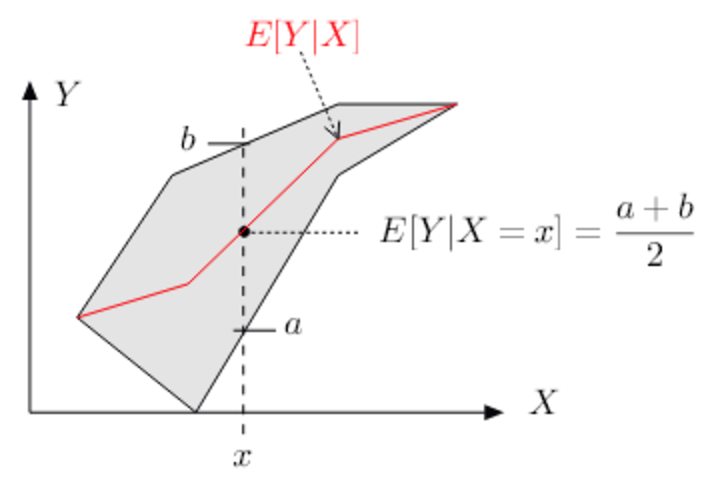
\includegraphics[width=8cm]{intro.jpg}
\end{center}
\end{minipage}}
